\documentclass[11pt,a4paper]{article}
\usepackage[T1]{fontenc}
\usepackage{lmodern,microtype,amsmath,amssymb,amsthm,booktabs,graphicx}
\usepackage[margin=25mm]{geometry}
\usepackage{xcolor,xurl,hyperref,fancyhdr,enumitem}
\usepackage[numbers,sort&compress]{natbib}
\hypersetup{colorlinks=true,linkcolor=blue!45!black,citecolor=blue!45!black,urlcolor=blue!45!black,
pdftitle={Face-Tail Diagnostics for Constraint Injection under Legendre p-Coarsening},pdfauthor={Shivam Gupta}}
\usepackage[font=small,labelfont=bf]{caption}
\setlength{\parskip}{3pt}
\setlength{\emergencystretch}{2em}
\setlength{\parindent}{1em}
\setlength{\headheight}{14pt}
\pagestyle{fancy}\fancyhf{}
\fancyhead[L]{\small Face-tail diagnostics for spectral coarsening}
\fancyhead[R]{\small S. Gupta}\fancyfoot[C]{\thepage}
\newtheorem{theorem}{Theorem}
\newtheorem{proposition}[theorem]{Proposition}
\newtheorem{corollary}[theorem]{Corollary}
\theoremstyle{remark}\newtheorem{remark}[theorem]{Remark}
\newcommand{\norm}[1]{\left\lVert #1\right\rVert}
\newcommand{\Pq}{\mathbb{P}_q}
\newcommand{\dd}{\,\mathrm{d}}
\newcommand{\T}{\mathcal{T}}
\graphicspath{{../figures/}}
\title{\bfseries Face-Tail Diagnostics for Constraint Injection\\under Legendre \(p\)-Coarsening}
\author{Shivam Gupta\\[3pt]\small Independent Researcher, Delhi, India\\
\small\href{mailto:shivam1720406@gmail.com}{shivam1720406@gmail.com}\\
\small ORCID: \href{https://orcid.org/0009-0009-4576-0138}{0009-0009-4576-0138}}
\date{17 October 2026}
\begin{document}
\maketitle
\begin{abstract}
Reducing the degree of a spectral element can violate a first-order reduction
constraint even when the source representation satisfies it. For Legendre modal
restriction, we express this transfer defect exactly through two endpoint values
of the discarded field. The resulting rank-at-most-two commutator gives an
explicit sharp tail-to-constraint amplification factor, an exact treatment of
inherited constraint error, and a low-cost test of a proposed coarsening. We
also quantify the field-error cost of the classical endpoint-preserving
\(H^1\) projector and identify a coefficient obstruction to repairing the
potential while retaining the independently restricted derivative. Tensor-product
extensions use face functions rather than two global scalars; nonaffine maps add
a separate multiplication commutator. Reproducible checks include exact rational
integration, 3,000 random polynomial transfers, 495 weighted singular-value
comparisons, 2,048 gauge-wave metric-component transfers, and periodic
discontinuous Galerkin scalar-wave evolutions. In the gauge-wave test, a field-only
threshold accepts 1,360 candidates, of which 224 violate an independently specified
constraint threshold; the exact joint test rejects those 224. Compatible projection
removes the immediate injection but does not consistently reduce later evolution
error. The contribution is an explicit diagnostic and transfer-cost analysis for
spectral adaptation, with direct relevance to first-order numerical-relativity
systems, rather than a new constraint-projection method or an Einstein evolution
scheme.
\end{abstract}
\noindent\textbf{Keywords:} numerical relativity; spectral adaptation; reduction constraints;
Legendre projection; discontinuous Galerkin methods; reproducible computation.

\smallskip\noindent\textbf{Code and data:}
\url{https://github.com/shi1720/legendre-face-tail}

\section{Introduction}
In a first-order evolution system, a field and its spatial derivative can be
independent numerical variables. For a scalar wave these are a potential
\(\psi\) and \(\Phi_i\), constrained by \(C_i=\partial_i\psi-\Phi_i=0\).
The generalized harmonic formulation has the analogous metric reduction
constraint \(C_{iab}=\partial_i g_{ab}-\Phi_{iab}\)
\cite{holst2004,lindblom2006}. A resolution change acts on both sides of this
relation. Restricting the variables separately need not give the same result as
differentiating the restricted potential.

This issue is relevant to adaptive spectral simulations even before the
time integrator or boundary conditions enter. Spectral adaptive mesh refinement
already monitors truncation, unresolved modes, and constraints
\cite{szilagyi2014}. SpECTRE supports local polynomial-degree changes within a
task-based discontinuous Galerkin (DG) framework \cite{kidder2017} that has
enabled binary black hole evolutions \cite{lovelace2025}. A useful adaptation
diagnostic should distinguish the constraint present before a transfer from the
constraint created by the transfer itself.

There is a particularly concrete implementation question. At the inspected
SpECTRE source revision, the constraint-based AMR criterion uses a coarsening
factor and explicitly suggests evaluating constraints after a lower-order
projection if choosing that factor proves difficult \cite{spectrecode}.
Here we analyze that prospective calculation for full-element Legendre
restriction. The question of inspecting a candidate coarse state is therefore
not new. Our purpose is to expose its exact structure, its worst-case
amplification, and the limitations of a compatible alternative.

The central result is that the injected reduction constraint depends on only
two discarded endpoint traces in one dimension. Small discarded \(L^2\) energy
does not determine these traces: equal-energy tails can inject zero constraint
or attain the sharp worst case. Once modal coefficients are available, parity
sums recover the complete new constraint without constructing a coarse nodal
state. The same sums also give the exact extra field-error cost of a familiar
endpoint-preserving \(H^1\) projection.

The paper makes three connected contributions. First, it gives a closed-form
transfer identity, its sharp finite-degree norm, and an exact separation of
inherited and newly created constraint error. Second, it relates this identity
to modal retention, endpoint preservation, and the classical compatible
projector, including an explicit repair-cost formula. Third, it tests the
diagnostic with independent algebra, nodal transfers, a metric-component
benchmark, and a time-dependent DG solver. The experiments distinguish an
instantaneous transfer guarantee from a claim about later waveform accuracy.

\section{Relation to established work}
Constraint projection and constraint-preserving boundary conditions have a
substantial numerical-relativity literature. Holst et al.\ construct optimal
projections using a field-space metric and demonstrate them for scalar fields
on a black hole background \cite{holst2004}. Lindblom et al.\ develop the
first-order generalized harmonic system with damping and boundary conditions
\cite{lindblom2006}; Rinne studies stable radiation-controlling boundary
conditions \cite{rinne2006}. These results concern the constrained evolution
problem and its boundary treatment. We study the algebra of a particular
change of representation. A local transfer diagnostic cannot replace those
methods.

Commuting projections are also classical. Projection-based interpolation
\cite{demkowicz2005} and finite element exterior calculus \cite{arnold2006}
organize approximation spaces so that projection respects differential
relations. The endpoint-preserving one-dimensional \(H^1\) projection used below
is an instance of this established approach. Neither its construction nor its
derivative-minimizing property is claimed as new.

Noncommutation of orthogonal polynomial truncation and differentiation is
explicitly treated by Rapisarda, van Waarde, and \c{C}amlibel
\cite{rapisarda2024}, including the parity-structured Legendre differentiation
matrix. Thus the existence of a commutator is not a novelty claim either.
We specialize that structure to reduction-constraint transfer and derive the
two-trace norm, sharp finite-tail gain, exact repair penalty, and candidate
decision test in a common notation. These are elementary consequences of
classical polynomial identities, supplied with proofs and independently
reproducible numerical checks.

Finally, Szil\'agyi's projected constraint error \cite[Sec.~6.1.4]{szilagyi2014}
projects derivative indices into grid-topology directions. That coordinate
projection differs from restricting polynomial degree. His work also shows
that removing a constraint-violating pile-up mode can \emph{reduce} constraints.
Our inherited-error formula permits that behavior: the inherited error and the
new commutator can cancel. The diagnostic does not assert that coarsening
always makes constraints larger.

\section{Transfer setting and exact face-tail identity}
\label{sec:identity}
Let \(I=[-1,1]\), let \(P_n\) be the standard Legendre polynomial normalized by
\(P_n(1)=1\), and write
\begin{equation}
 u(\xi)=\sum_{n=0}^{N}a_nP_n(\xi),\qquad
 \T_q u=\sum_{n=0}^{q}a_nP_n(\xi),\qquad 0\le q<N.
 \label{eq:truncation}
\end{equation}
Here \(\T_q\) is the continuous unweighted \(L^2(I)\) projector, and
\(D=\partial_\xi\). The normalization is
\begin{equation}
 \norm{u}^2=\sum_{n=0}^{N}\frac{2a_n^2}{2n+1}.
 \label{eq:norm}
\end{equation}
All fields are real; the complex case follows with conjugation. An affine
physical element of length \(h\) has \(\partial_x=(2/h)D\).

For a source pair \((u,v)\) with logical reduction constraint \(C=Du-v\),
componentwise restriction gives
\begin{equation}
 C_q=D\T_q u-\T_q v
     =\T_q C+c_q(u),\qquad
 c_q(u):=(D\T_q-\T_q D)u.
 \label{eq:inherited}
\end{equation}
The first term is inherited constraint error. The second is introduced solely
by restriction. This decomposition is exact and does not assume \(C=0\).

Define the discarded parity sums and endpoint traces by
\begin{equation}
 s_p=\sum_{\substack{q<n\le N\\n\equiv p\ (2)}}a_n,\quad p\in\{0,1\},
 \qquad r=u-\T_q u,\qquad e_\pm=r(\pm1).
 \label{eq:tail}
\end{equation}
Then \(s_0=(e_++e_-)/2\) and \(s_1=(e_+-e_-)/2\).

\begin{theorem}[Two-trace transfer identity]
\label{thm:identity}
For the transfer in \eqref{eq:truncation},
\begin{align}
 c_q(u)&=-\sum_{k=0}^{q}(2k+1)s_{1-(k\bmod2)}P_k,
 \label{eq:identity}\\
 \norm{c_q(u)}^2
 &=2\sum_{k=0}^{q}(2k+1)s_{1-(k\bmod2)}^2.
 \label{eq:injectionnorm}
\end{align}
The discarded-tail-to-constraint map has rank at most two. For \(q\ge1\)
and \(N\ge q+2\), its rank is exactly two.
\end{theorem}
\begin{proof}
Since \(D\T_q u\in\mathbb P_{q-1}\),
\(c_q=-\T_q Dr\). For \(k\le q\), integration by parts and Legendre
orthogonality give
\begin{equation}
 \int_{-1}^{1}Dr\,P_k\dd\xi
 =e_+-(-1)^k e_- -\int_{-1}^{1}r\,DP_k\dd\xi
 =e_+-(-1)^k e_-.
\end{equation}
The last integral vanishes because \(DP_k\in\mathbb P_{q-1}\).
Multiplication by \((2k+1)/2\) gives the coefficient of \(\T_q Dr\),
which proves \eqref{eq:identity}. Orthogonality gives
\eqref{eq:injectionnorm}. Even and odd discarded modes excite disjoint retained
parities. Both are nonempty under the stated degree conditions, proving rank two.
\end{proof}

The proof uses only the residual's orthogonality and its endpoint traces. The
identity therefore extends to \(u\in H^1(I)\) with \(r=u-\T_q u\), without
requiring a convergent endpoint evaluation of an infinite coefficient series.
The finite polynomial setting remains the computational setting of this paper.
For \(q=0\), or for a single discarded mode, the rank can be one.

\begin{corollary}[Exact prospective constraint test]
\label{cor:guard}
On an affine one-dimensional element, independently restricting \(u\) and a
physical derivative variable \(\Phi\) gives
\begin{equation}
 C_{x,q}=\T_q C_x+\frac{2}{h}c_q(u),\qquad C_x=\frac{2}{h}Du-\Phi.
 \label{eq:physical}
\end{equation}
Its physical squared norm is \((h/2)\norm{C_{x,q}}^2\). Testing this quantity
against a specified squared tolerance is equivalent, in exact arithmetic, to
forming the coarse fields and differentiating them.
\end{corollary}

Adding \(\norm{\T_q C_x}\) and \((2/h)\norm{c_q}\) gives a sufficient
bound, but loses possible cancellation. The implementation retains the signed
coefficients in \eqref{eq:physical}. Monitoring only the pre-transfer constraint
cannot detect the injection from an initially constraint-satisfying state.

\section{Sharp amplification and the cost of compatible transfer}
\label{sec:sharp}
\subsection{A sharp finite-degree bound}
Let
\begin{equation}
 A_{q,p}=2\sum_{\substack{0\le k\le q\\k\not\equiv p\ (2)}}(2k+1),\qquad
 B_{Nq,p}=\frac12\sum_{\substack{q<n\le N\\n\equiv p\ (2)}}(2n+1).
 \label{eq:ab}
\end{equation}
An empty sum is zero.
\begin{theorem}[Sharp tail amplification]
\label{thm:gain}
The exact operator norm from discarded field \(L^2\) norm to injected
constraint \(L^2\) norm is
\begin{equation}
 G_{Nq}=\max_{p\in\{0,1\}}\sqrt{A_{q,p}B_{Nq,p}},\qquad
 \norm{c_q(u)}\le G_{Nq}\norm{u-\T_q u}.
 \label{eq:gain}
\end{equation}
Equality is attained by a tail supported on a maximizing parity with
\(a_n\) proportional to \((2n+1)/2\) on that parity.
\end{theorem}
\begin{proof}
Set \(E_p=\sum_{n>q,\ n\equiv p}2a_n^2/(2n+1)\).
Weighted Cauchy--Schwarz gives \(s_p^2\le B_{Nq,p}E_p\), with equality
for the stated coefficients. Equation~\eqref{eq:injectionnorm} becomes
\(\norm{c_q}^2=\sum_p A_{q,p}s_p^2\).
Bounding each product by \(\max_p A_{q,p}B_{Nq,p}\) times \(E_p\), then
summing, proves the bound. Concentrating the tail energy on a maximizing
parity attains it.
\end{proof}

For fixed \(q\), the gain grows linearly with \(N\). An \(L^2\)-only
infinite-tail assumption cannot bound the transfer constraint uniformly.
For a physical element the ratio between physical constraint norm and physical
discarded-field norm is \((2/h)G_{Nq}\). This explains why the same coefficient
tail can become more consequential on smaller elements.

The gain is a worst-case statement, not a typical-case prediction. At
\((N,q)=(24,8)\), a unit-norm maximizing tail injects \(108.995413\ldots\),
whereas a normalized multiple of \(P_9-P_{11}\) injects zero. The latter tail
has zero traces at both endpoints. A tail-energy threshold discards the
information that distinguishes these cases (Fig.~\ref{fig:cancellation}).

\begin{figure}[t]
\centering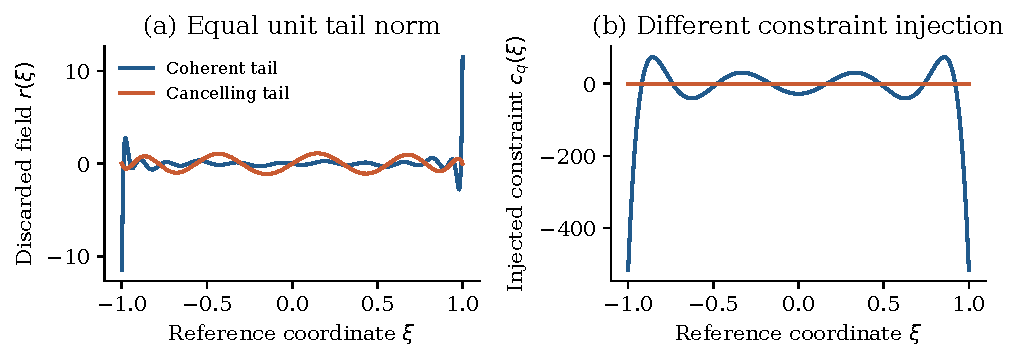
\includegraphics[width=\linewidth]{tail_cancellation.pdf}
\caption{Two discarded tails at \(N=24,q=8\), each with unit continuous
\(L^2\) norm. The coherent tail attains the sharp gain; the cancelling tail
has zero endpoint traces and injects no logical reduction constraint.}
\label{fig:cancellation}
\end{figure}

\subsection{Classical compatible projection in two-mode form}
For \(q\ge1\), let \(m_p\) be the largest integer at most \(q\) of parity
\(p\), and define
\begin{equation}
 H_q u=\T_q u+s_0P_{m_0}+s_1P_{m_1}.
 \label{eq:h1}
\end{equation}
This is the endpoint-preserving \(H^1\) projector, expressed through the
same two tail sums. It is a classical compatible approximation operator;
the following properties clarify what it changes in this transfer setting.

\begin{proposition}[Compatibility, retained modes, and field penalty]
\label{prop:h1}
For \(q\ge1\),
\begin{align}
 (H_q u)(\pm1)&=u(\pm1), &D H_q u&=\T_{q-1}Du,
 \label{eq:h1properties}\\
 \norm{u-H_q u}^2
 &=\norm{u-\T_q u}^2+
 \frac{2s_0^2}{2m_0+1}+\frac{2s_1^2}{2m_1+1}.
 \label{eq:cost}
\end{align}
It minimizes \(\norm{D(u-w)}\) among \(w\in\Pq\) with either endpoint
anchored to \(u\), and \(\norm{D H_q u}\le\norm{Du}\).
For \(q\ge2\), it uniquely preserves both endpoint values and every
Legendre coefficient through degree \(q-2\). For \(q=1\), its constant
coefficient can change.
\end{proposition}
\begin{proof}
At the endpoints, \(P_{m_0}(1)=P_{m_0}(-1)=1\) and
\(P_{m_1}(1)=-P_{m_1}(-1)=1\), so the correction restores \(e_\pm\).
The classical derivative identity
\(DP_n=\sum_{k<n,\ n-k\ \mathrm{odd}}(2k+1)P_k\)
\cite{dlmf,rapisarda2024} shows that differentiating the two correction
modes adds precisely the tail contributions of \(Du\) through degree
\(q-1\). Hence \(D H_q u=\T_{q-1}Du\).
Equation~\eqref{eq:cost} follows because the discarded tail and the two
retained correction modes are mutually orthogonal. Every polynomial in
\(\mathbb P_{q-1}\) is the derivative of a unique endpoint-anchored
polynomial in \(\Pq\). Orthogonal projection of \(Du\) therefore proves
minimality and contraction. Finally, with coefficients through \(q-2\)
fixed, the two endpoint equations uniquely determine the last two
coefficients and give \eqref{eq:h1}.
\end{proof}

For a consistent scalar-wave state, the transfer
\begin{equation}
 u\mapsto H_q u,\qquad \Pi\mapsto\T_q\Pi,\qquad
 \Phi\mapsto\T_{q-1}\Phi
 \label{eq:compatibletransfer}
\end{equation}
preserves the reduction constraint on an affine element. It contracts the
flat-space wave energy \(\tfrac12\int(\Pi^2+\Phi^2)\dd x\), since each
derivative variable is orthogonally projected. This statement concerns
consistent source data and this particular energy. It does not apply to a
general relativistic symmetrizer or imply contraction of an energy containing
an independent \(u^2\) term.

For inconsistent data the new logical constraint is
\(\T_{q-1}(Du-v)\), not necessarily zero. Endpoint preservation applies
to \(u\); it does not preserve characteristic combinations involving
\(\Pi\) and \(\Phi\). These distinctions matter at DG interfaces.

\begin{proposition}[Obstruction to potential-only repair]
\label{prop:obstruction}
There exists \(w\in\Pq\) satisfying \(Dw=\T_q Du\) if and only if
\(s_{1-(q\bmod2)}=0\). When this condition holds, anchoring one endpoint
gives \(w=H_q u\), which also preserves the other endpoint.
\end{proposition}
\begin{proof}
The coefficient of \(P_q\) in \(\T_q Du\) is
\((2q+1)s_{1-(q\bmod2)}\), whereas \(Dw\) has degree at most \(q-1\).
Its vanishing is necessary and sufficient. When it vanishes,
\(\T_q Du=\T_{q-1}Du\), so Proposition~\ref{prop:h1} supplies the
unique endpoint-anchored primitive.
\end{proof}

Thus changing only the potential cannot generically repair the constraint
while retaining all independently restricted derivative coefficients.
Setting \(\Phi=D\T_q u\) repairs the algebraic constraint instead, but
alters derivative information and need not contract wave energy. Neither
repair is universally preferable to rejecting the coarsening.

\begin{figure}[t]
\centering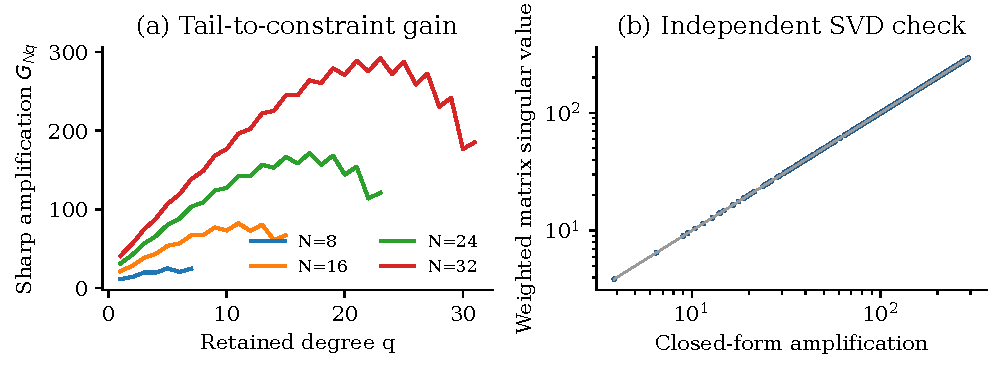
\includegraphics[width=\linewidth]{sharp_gain.pdf}
\caption{Sharp finite-tail gain. Left: its dependence on source and retained
degrees. Right: closed-form and independently assembled weighted-matrix
singular values for all 495 pairs \(3\le N\le32,1\le q<N\). The largest
relative difference is \(7.1\times10^{-16}\).}
\label{fig:gain}
\end{figure}

\section{Tensor products, mappings, and implementation}
\label{sec:implementation}
\subsection{Face functions on a tensor-product element}
Let \(u=\sum_{\boldsymbol n}a_{\boldsymbol n}\prod_jP_{n_j}(\xi_j)\),
with degree caps \(N_j\), and let
\(\T_{\boldsymbol q}=\prod_j\T_{q_j}^{(j)}\). Fix direction \(i\).
For every retained transverse multi-index \(\boldsymbol\ell\), define
\begin{equation}
 s_{i,p,\boldsymbol\ell}
 =\sum_{\substack{q_i<n_i\le N_i\\n_i\equiv p\ (2)}}
 a_{(\boldsymbol\ell,n_i)}.
 \label{eq:tensortail}
\end{equation}
Here \((\boldsymbol\ell,n_i)\) inserts \(n_i\) in slot \(i\).
Because transverse restriction commutes with \(D_i\),
\begin{equation}
 (D_i\T_{\boldsymbol q}-\T_{\boldsymbol q}D_i)u
 =-\sum_{\boldsymbol\ell}\sum_{k=0}^{q_i}
 (2k+1)s_{i,1-(k\bmod2),\boldsymbol\ell}
 P_k(\xi_i)\prod_{j\ne i}P_{\ell_j}(\xi_j).
 \label{eq:tensoridentity}
\end{equation}
Its squared norm follows by multiplying every squared coefficient by
\(\prod_j2/(2\ell_j+1)\), with \(\ell_i=k\).
There are two \emph{face functions} per direction, not two numbers for a
whole multidimensional element. The directional rank is at most
\(2\prod_{j\ne i}(q_j+1)\). The software verifies both two- and
three-dimensional cases. A tensor-product compatible projection also requires
different scalar and derivative spaces, as in compatible discretization
theory; a componentwise use of \eqref{eq:h1} in every variable is not
automatically a commuting multidimensional transfer.

\subsection{Why nonaffine physical maps require another term}
For a one-dimensional map with positive Jacobian \(J(\xi)\), write
\(v=J^{-1}\). A consistent physical derivative is \(\Phi=vDu\).
Independent physical-field projection satisfies the exact functional identity
\begin{equation}
 vD\T_q u-\T_q(vDu)
 =v\,c_q(u)+[v,\T_q]Du,
 \quad [v,\T_q]f=v\T_q f-\T_q(vf).
 \label{eq:mapping}
\end{equation}
The second term vanishes for constant \(J\). It does not vanish for a
general mapped element, and its norm is not determined by the two traces of
the discarded potential. Moreover, interpolation of \(vDu\) on a finite
source grid introduces an additional representation error if that product is
not polynomial. Equation~\eqref{eq:mapping} describes continuous projection;
a mapped nodal code must also account for that aliasing.

A counterexample is \(u=P_9-P_{11}\), \(q=8\), and
\(x=\xi+\alpha\xi^2/2\). The affine face-tail term vanishes identically,
but projection of the rational physical derivative gives logical-measure
constraint norms approximately \(0.01643\), \(0.16258\), and \(0.95920\)
for \(\alpha=0.1,0.3,0.6\), respectively. Figure~\ref{fig:mapping}
shows this failure of an affine-only diagnostic. A practical mapped-element
implementation can evaluate a candidate physical coarse state directly, or
separately bound the mapping commutator. Neither shortcut is supplied by the
rank-two theorem.

\subsection{Connection to SpECTRE and numerical norms}
The inspected SpECTRE revision is
\texttt{d57433e93984c238a144f83411eda9f125759812}
\cite{spectrecode}. In \texttt{Projection.cpp}, the full-segment,
non-massive projection branch forms a modal-to-nodal matrix, truncates or
zero-pads modal coefficients, and applies a nodal-to-modal matrix.
The pure \(p\)-projection route delegates to this branch. For a polynomial
represented exactly at source nodes, this gives
\begin{equation}
 R_{Nq}=V_q\,[I_{q+1}\ 0]V_N^{-1},
 \label{eq:nodal}
\end{equation}
where \(V_N\) and \(V_q\) are the source and target Legendre Vandermonde
matrices. Our tests independently implement \eqref{eq:nodal} for all four
Gauss/Gauss--Lobatto source-target combinations. This is source-level
alignment and independent reimplementation, not a linked SpECTRE run or an
upstream contribution.

Once the modal coefficients are available, forming parity suffix sums costs
\(O(N)\) per one-dimensional line. Every candidate \(q\) then requires
constant work for the injected norm and the two-mode field penalty, or
\(O(q)\) to assemble the complete residual including inherited coefficients.
A nodal-to-modal transform still has its usual cost when coefficients are
not already available. No end-to-end runtime speedup is claimed.

The theorem uses continuous norms. Gauss--Lobatto quadrature with \(q+1\)
nodes does not integrate the square of a degree-\(q\) polynomial exactly.
Consequently a lumped nodal norm of \(C_q\) need not equal
\eqref{eq:injectionnorm}. The supplied implementation uses exact modal norm
weights. It does not silently substitute a quadrature norm.

\section{Computational validation}
\label{sec:experiments}
All computations are deterministic and use double precision unless exact
rational arithmetic is specified. Raw results, seeds, scripts, and the
environment record accompany the code. The experiments address algebraic
correctness, candidate screening, and subsequent evolution separately.

\subsection{Independent algebra and nodal tests}
Seven automated test groups verify the inherited-error identity, the
prospective decision with inherited error, all four nodal quadrature
combinations, endpoint and derivative projection properties, sharpness,
exact rational polynomial integration, and tensor-product identities.
The rational check integrates monomial representations obtained from the
closed-form Legendre polynomial coefficients; it does not reuse the
implemented Legendre differentiation routine. It covers the 119 degree pairs
\(2\le N\le15,0\le q<N\).

A separate random experiment uses \(N\in\{8,16,24,32,48\}\),
\(q\in\{2,4,6\}\), and 200 coefficient vectors per pair, generated with
seed 6602027 and scaled by \((n+1)^{-2}\). Direct differentiation and the
two-trace formula differ by at most \(4.45\times10^{-16}\) in any modal
coefficient across 3,000 cases. The computed gains are checked against
weighted singular values of independently assembled differentiation and
restriction matrices for 495 degree pairs (Fig.~\ref{fig:gain}).
These tests support implementation correctness; the mathematical guarantee
comes from the proofs rather than from a finite test count.

\subsection{Gauge-wave metric-component transfers}
The standard gauge-wave test represents flat spacetime in nontrivial
coordinates \cite{alcubierre2004}. We use one metric component
\begin{equation}
 g_{xx}(x,t)=H(x,t)=1-0.1\sin\bigl(2\pi(x-t)\bigr),
 \qquad \Phi_{xxx}=\partial_xH.
 \label{eq:gaugewave}
\end{equation}
This experiment transfers a component and its reduction variable. It does
not evolve Einstein's equations or test the full harmonic gauge constraint.
On each patch, \(H\) is first projected to degree \(N=24\) by 96-point
Gauss quadrature, and its derivative is obtained by differentiating that
polynomial. Thus the source polynomial pair satisfies the reduction
constraint exactly up to arithmetic error; the analytic-to-polynomial
approximation is separate from the transfer defect.

We use patch length \(h=0.5\), eight centers from \(-0.875\) to
\(0.875\), 32 phases \(t=j/32\), and target degrees
\(q\in\{2,3,4,5,6,8,10,12\}\), giving 2,048 transfer candidates.
These are overlapping test patches and deterministic phases, not
independent observational samples. Predicted and directly measured
physical constraint norms differ by at most \(1.12\times10^{-16}\).
Compatible transfer produces a largest measured reduction constraint of
\(5.27\times10^{-17}\) and a largest endpoint error of
\(2.23\times10^{-16}\).

Figure~\ref{fig:gauge} compares field and constraint errors. To illustrate
screening, impose a physical discarded-field tolerance \(\eta=10^{-4}\)
and a physical constraint tolerance \(\varepsilon=10^{-3}\).
The field-only test accepts 1,360 candidates. Of these, 224 have
post-transfer constraint norm above \(\varepsilon\). The joint exact
test accepts the remaining 1,136. At the same constraint tolerance, field
tolerances \(10^{-3}\) and \(10^{-5}\) accept 1,680 and 1,072
candidates, with 544 and zero constraint violations, respectively.
These thresholds are illustrative choices in nondimensional units; the
counts are not an estimated failure probability or a tuned optimal policy.

\begin{figure}[t]
\centering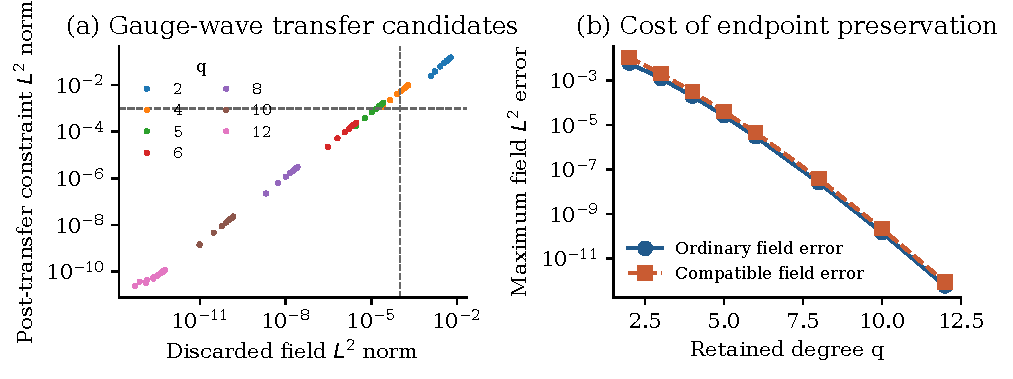
\includegraphics[width=\linewidth]{gauge_transfer.pdf}
\caption{Gauge-wave metric-component transfers. Left: discarded field error
does not alone determine the reduction constraint. Dashed lines show the
illustrative tolerances \(\eta=10^{-4}\) and \(\varepsilon=10^{-3}\).
Right: compatible endpoint preservation has a larger maximum field error,
consistent with the exact orthogonal penalty in \eqref{eq:cost}.}
\label{fig:gauge}
\end{figure}

\subsection{Periodic scalar-wave evolution}
To examine what an instantaneous guarantee does and does not imply, we
implement an independent one-dimensional DG solver for
\begin{equation}
 \partial_t\psi=-\Pi,\qquad
 \partial_t\Pi=-\partial_x\Phi,\qquad
 \partial_t\Phi=-\partial_x\Pi+\gamma_2(\partial_x\psi-\Phi),
 \quad\gamma_2=1.
 \label{eq:evolution}
\end{equation}
The domain is periodic, \([-1,1]\), with eight equal elements. A strong-form
LGL nodal DG discretization uses upwind acoustic interface fluxes based on
\(w_\pm=\Pi\pm\Phi\), the speed-\(\pm1\) characteristics of the
undamped acoustic subsystem. The damping term, including its potential
derivative, is evaluated in the element volume. These acoustic combinations
are not the characteristic variables of the complete principal matrix when
\(\gamma_2\ne0\). The zero-speed potential receives no interface flux
lift. Fourth-order
Runge--Kutta integration uses nominal step
\(\Delta t=0.12h/(p+1)^2\), shortened uniformly within each time interval
to land exactly on the transfer and final times. Every transfer experiment
is repeated with half this step.

Initial data are a right-moving smooth wave,
\begin{equation}
 \psi(x,0)=\sin(\pi x)+0.2\cos(3\pi x),\quad
 \Pi(x,0)=\Phi(x,0)=\pi\cos(\pi x)-0.6\pi\sin(3\pi x).
 \label{eq:initial}
\end{equation}
The analytic solution is obtained by replacing \(x\) with \(x-t\).
The fine run uses degree 14 until \(t_*=0.25\), when all elements are
coarsened to degree 4, 6, or 8. We compare ordinary componentwise
truncation, truncation followed by \(\Phi\leftarrow\partial_x\T_q\psi\)
(reset), and \eqref{eq:compatibletransfer}. All continue to \(t=1\).
Constraint and energy norms are integrated exactly in the modal basis;
field error relative to the analytic wave is integrated at 48 independent
Gauss points per element. Error is therefore measured between functions,
not merely at target interpolation nodes.

\begin{table}[t]
\centering\small
\caption{Degree-14 to degree-6 transfer at \(t=0.25\). Values use the
nominal step. \(\Delta E\) is the immediate wave-energy change;
\(e_\psi\) is the physical continuous \(L^2\) field error.}
\label{tab:transfer}
\begin{tabular}{lrrrr}
\toprule
Transfer & \(\norm{C}_{t_*^+}\) & \(\Delta E\) & \(e_\psi(t_*^+)\) & \(e_\psi(1)\)\\
\midrule
Truncate & \(1.8883\!\times\!10^{-4}\) & \(-1.1923\!\times\!10^{-10}\) & \(1.1585\!\times\!10^{-6}\) & \(6.8888\!\times\!10^{-6}\)\\
Reset & \(1.8296\!\times\!10^{-14}\) & \(+3.0844\!\times\!10^{-5}\) & \(1.1585\!\times\!10^{-6}\) & \(6.5014\!\times\!10^{-6}\)\\
Compatible & \(1.3150\!\times\!10^{-13}\) & \(-8.3580\!\times\!10^{-9}\) & \(1.7754\!\times\!10^{-6}\) & \(6.6662\!\times\!10^{-6}\)\\
\bottomrule
\end{tabular}
\end{table}

The pre-transfer constraint is \(3.22\times10^{-13}\). Ordinary
coarsening injects global constraints of approximately \(1.4025\times10^{-2}\),
\(1.8883\times10^{-4}\), and \(1.3147\times10^{-6}\) at target degrees
4, 6, and 8, matching the face-tail prediction. Reset and compatible
transfer remove the immediate injection to arithmetic accuracy, up to
inherited error. At degree 6, however, reset adds \(3.08\times10^{-5}\)
wave energy, while compatible transfer loses \(8.36\times10^{-9}\)
(Table~\ref{tab:transfer}). This is a measured example of energy addition
by derivative resetting, not a claim that reset always adds energy.

After continued evolution, compatible transfer has a larger constraint norm
than ordinary truncation in these tests. At degree 6 the final values are
approximately \(3.90\times10^{-4}\) and \(3.52\times10^{-4}\), respectively.
The immediate algebraic improvement therefore does not persist as a
uniform dynamical improvement. The DG interface treatment and the coarse
evolution can generate fresh reduction error. All three methods converge
rapidly as the target degree increases, and reset gives the lowest final
field error among the three in this particular experiment. These results
support screening or quantifying a transfer; they do not establish a
preferred replacement evolution method.

\begin{figure}[t]
\centering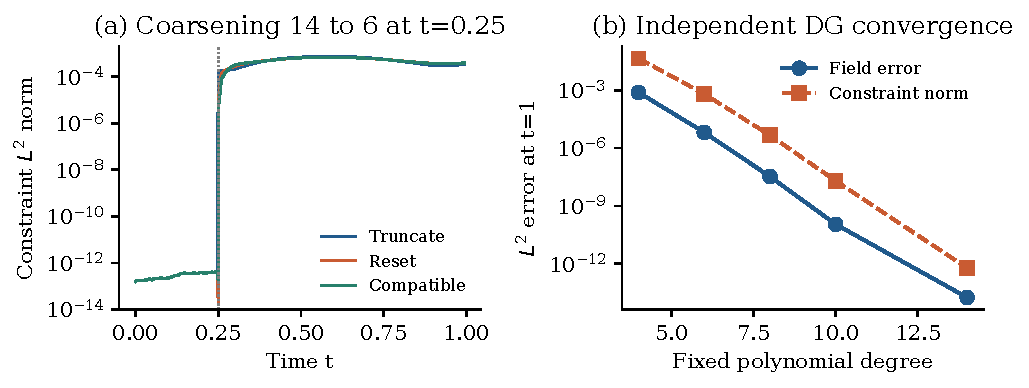
\includegraphics[width=\linewidth]{wave_evolution.pdf}
\caption{Left: constraint evolution for the degree-14 to degree-6
experiment, with the half-step runs shown. Compatible transfer and resetting
suppress the instantaneous jump at \(t=0.25\), but later coarse evolution
generates constraints again. Right: fixed-degree, no-transfer convergence
against the analytic wave at \(t=1\).}
\label{fig:evolution}
\end{figure}

\begin{table}[t]
\centering\small
\caption{Independent fixed-degree DG convergence at \(t=1\), with
\(\Delta t\le0.06h/(p+1)^2\), without coarsening.}
\label{tab:convergence}
\begin{tabular}{rrr}
\toprule
Degree \(p\) & Field error \(\norm{\psi_h-\psi}\) & Constraint norm \(\norm{C_h}\)\\
\midrule
4 & \(7.7048\times10^{-4}\) & \(4.4701\times10^{-2}\)\\
6 & \(6.4971\times10^{-6}\) & \(6.3812\times10^{-4}\)\\
8 & \(3.3188\times10^{-8}\) & \(4.5829\times10^{-6}\)\\
10 & \(1.1076\times10^{-10}\) & \(1.9802\times10^{-8}\)\\
14 & \(1.7610\times10^{-14}\) & \(5.9054\times10^{-13}\)\\
\bottomrule
\end{tabular}
\end{table}

The independent fixed-degree convergence test in
Table~\ref{tab:convergence} verifies the evolution implementation against
the analytic solution. Halving the nominal time step in the transfer runs
changes the degree-6 final field errors by less than \(1.1\times10^{-11}\)
in absolute norm. The paired time-step results and all degree-4 and
degree-8 results are included in the repository.

\begin{figure}[t]
\centering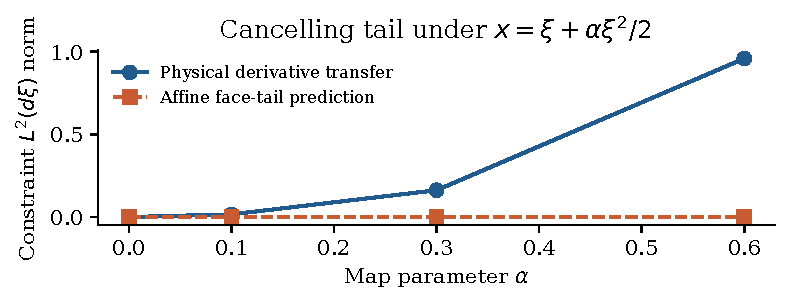
\includegraphics[width=.83\linewidth]{mapped_failure.pdf}
\caption{Nonaffine mapping counterexample. The discarded potential
\(P_9-P_{11}\) has zero face-tail injection at \(q=8\), but the
physical derivative projection has a nonzero constraint when the inverse
Jacobian varies. Norms here use \(d\xi\); 256-point Gauss quadrature
evaluates the rational derivative. The affine baseline is about
\(5.7\times10^{-12}\) from numerical cancellation.}
\label{fig:mapping}
\end{figure}


\subsection{Computational assistance and verification provenance}
OpenAI Codex was used to assist with topic development and literature discovery,
mathematical derivation, implementation of the reference operators and tests,
execution and analysis of numerical experiments, and manuscript drafting.
The numerical results reported here were produced by the executable Python
scripts in the public repository. Figures were generated from those results
with Matplotlib; they are not generative illustrations. The algebraic checks,
independent nodal calculations, singular-value comparisons and convergence
checks are specified above so that a reader can audit the computations without
relying on generated prose. Automated checks do not replace scientific review
by the named author or establish exhaustive novelty.

\section{Use in adaptation and scope of the result}
A candidate coarsening can now be assessed without conflating field fidelity
and reduction consistency. In the affine setting, first compute the
discarded-field norm and the prospective constraint in
Corollary~\ref{cor:guard}. Reject the candidate if either prescribed
tolerance is exceeded. If endpoint preservation is required instead,
\eqref{eq:cost} gives the compatible field error exactly before committing
to the alternative transfer. A decision to modify the state should remain
separate from the decision to reduce degree.

This test concerns only a specified instant and specified constraints.
In generalized harmonic evolution, satisfying \(C_{iab}\) does not imply
satisfaction of the harmonic gauge, Hamiltonian, momentum, or all
constraint-propagation relations. The physical characteristic data and
symmetrizer also depend on the metric. A scalar flat-space energy argument
does not certify those structures. In particular, the metric-component
test in Sec.~\ref{sec:experiments} is a controlled transfer benchmark,
not evidence of an accurate binary black hole waveform.

The mapped counterexample limits direct deployment: a two-trace guard
alone is unsuitable for a general curved or moving mesh. A production
SpECTRE contribution would need integration into its actual AMR
projectors, mapped tensor variables, constraints, and boundary-data
recalculation. Independent comparisons against prospective coarse-state
evaluation should precede any replacement of an existing criterion.
No such production integration or strong-field evolution has been performed
here. The available code is a research reference implementation.

The practical opportunity is modest but concrete. Spectral simulation
software can expose the predicted constraint jump and the compatible field
penalty as adaptation diagnostics, including when candidate resolutions
are proposed by automated tooling. Such diagnostics could support
verification services for simulation workflows across scientific and
engineering applications. This study does not quantify cost savings,
customer demand, or patentability; its commercial value would depend on
integration and validated reductions in failed or over-resolved runs.

\section{Conclusion}
For full-element Legendre restriction, two discarded endpoint traces
determine the complete newly introduced first-order reduction constraint
in one dimension. The identity supplies a sharp finite-degree
amplification factor, an exact inherited-error decomposition, and a
prospective constraint test. The same parity sums quantify the field
penalty of a classical compatible projector and expose when a
potential-only repair is impossible.

The computational evidence verifies these transfer statements while
showing their limits. Field-only screening admits constraint-violating
coarsenings in a deterministic metric-component test, nonaffine maps add
an independent defect, and eliminating the immediate jump does not
guarantee a better evolved solution. The resulting contribution is a
small, explicit component for auditable spectral adaptation, with clear
conditions under which it can be used and tested.

\section*{Reproducibility and availability}
The repository contains the reference operators, automated tests,
experiment and figure scripts, raw CSV results, environment metadata,
and this manuscript's source. The code is released under the MIT license.
From the repository root:
\begin{verbatim}
python -m pip install -r requirements.txt
PYTHONPATH=src python -m unittest discover -s tests -v
python experiments/run.py
python experiments/figures.py
cd paper && tectonic main.tex
\end{verbatim}
The reported environment uses Python with NumPy 1.26.4, SciPy 1.13.1,
Matplotlib 3.9.4, and pandas. No external simulation data are needed.
Source references to SpECTRE are pinned to the revision identified in
Sec.~\ref{sec:implementation}. Floating-point agreement tolerances and
the distinction between continuous and nodal norms are documented in
the tests. The manuscript is a research working paper and has not been
peer reviewed.


\section*{Declaration of generative AI and AI-assisted technologies}
During preparation of this work, OpenAI Codex was used for research assistance,
code development, computational analysis and manuscript preparation, as
specified in the computational provenance subsection. This disclosure describes
substantive assistance beyond spelling or grammar correction. The tool is not
an author. After using the tool, the author reviewed the content, approved
the manuscript and disclosure, and accepts responsibility for the work.

\bibliographystyle{unsrtnat}
\bibliography{references}
\end{document}
